% \usepackage{graphicx}
% \usepackage{listings, listings-rust}
% \usepackage{multirow}
% 
% \usepackage{xcolor,colortbl}
% \usepackage{cite}
% \usepackage{mathtools}
% \usepackage{amsmath}
% \usepackage{cleveref}
% \usepackage{proof}
% \usepackage{algpseudocode}
% \usepackage{float}
% \usepackage{booktabs} % for borders and merged ranges
% \usepackage{soul}% for underlines
% %\usepackage[table]{xcolor} % for cell colors
% \usepackage{changepage}
% \usepackage{parcolumns}
% \usepackage{threeparttable} % for wide tables
% \setlength{\textfloatsep}{14pt}
% \begin{document}
\chapter[Equivalence Checking of a libm Port]{Equivalence Checking of a libm Port\protect\footnotemark} \footnotetext{Adapted with permission from \textit{Equivalence Checking of a libm Port}, TACAS 2025~\cite{2025_tacas_brg}. Reproduced with permission from Springer Nature.}
\label{chap4}
\setupuuchapterbib
% \chapter{Equivalence Checking of a libm Port}\footnote{Adapted with permission from ...}
% \label{chap4}
%\thanks{Supported in part by ...}
%
%\author{Mark Baranowski \and Zvonimir Rakamari\'c}
%\institute{
%  School of Computing, University of Utah, Salt Lake City, USA \\
%  \email{\{baranows,zvonimir\}@cs.utah.edu}
%}
%
%
% \maketitle
%
% \begin{abstract}
%
% \end{abstract}
%
\vspace{-2.5em}
\section{Introduction}
Rust is a modern programming language focused on safety and native performance.
%
Due to Rust's novelty, it has been reliant on libraries written in other programming languages, often C, to provide many core functions.
%
However, languages such as C do not have the same safety guarantees provided by Rust and are thus unsafe to use inside Rust.
%
Many libraries provide safe Rust bindings to such C language libraries.
%
But this requires the library developer to completely contain any potential unsafety within their library.
%
Additionally, the foreign code used in this process may not be as optimizable as native Rust code, such as allowing inlining, and may inhibit debugging of such programs from Rust.

An alternative option is to instead port the library code from the source language to Rust.
%
This has the upside of making the library native for Rust programs, and limits or eliminates unsafe code used inside the library.
%
Nonetheless, such ports may not always be correct because of subtleties related to the source programming language.
%
This can be exacerbated by the usage of floating-point arithmetic, which introduces additional subtleties that may not be as well known.
%
Moreover, languages may not have complete support for floating-point arithmetic, which may lead to bugs that are difficult to detect within the language itself.

Formal equivalence checking can provide a solution here because it can show that the original-language program matches the behavior of the program ported to the target programming language.
%
In this work, we apply the SMACK (please refer to \cref{sec:smackground}) software verifier to the Rust-language port of the \texttt{musl} C-language math library.
%
SMACK is a software verifier that can work with both C and Rust language programs at once.
%
We give our experiences using SMACK to show the equivalence of these programs and our extensions to the SMACK verifier to help show equivalence of more programs.
\section{Background}
In this section, we give some needed background on floating-point arithmetic.
% \subsection{SMACK}
% \begin{figure}[tb]
%   \centering
%   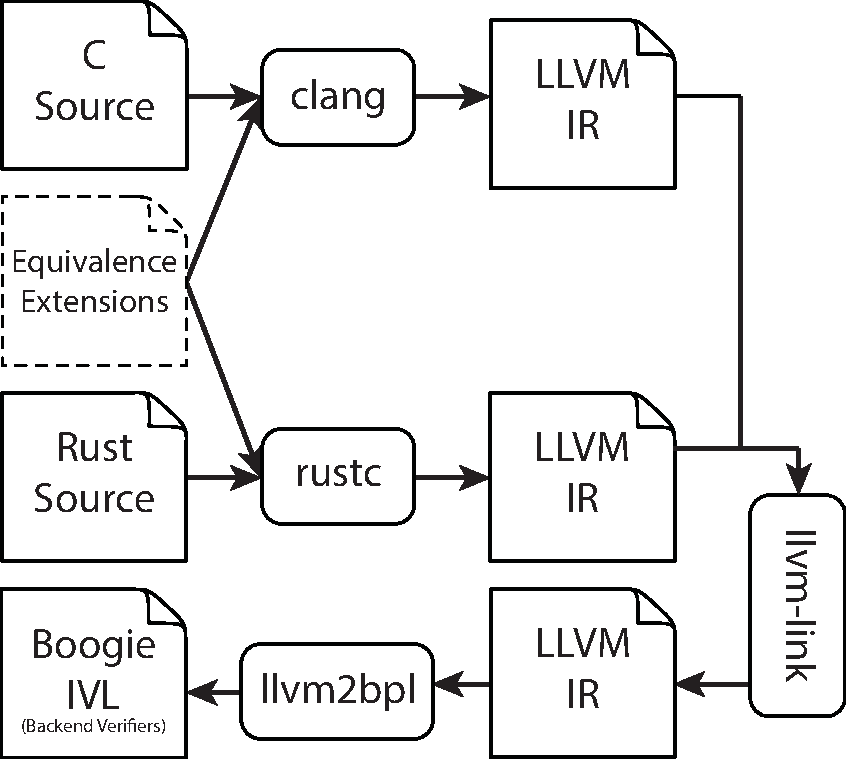
\includegraphics[width=0.92\textwidth]{chap4/fig/SmackEquiv.pdf}
%   \caption{Toolflow of SMACK.}
%   \label{fig:toolflow}
% \end{figure}

% SMACK~\cite{smack} is a software verification toolchain that translates
% LLVM IR code into Boogie intermediate verification language~\cite{boogie}, which
% is in turn verified using back-end Boogie verifiers such as the
% Boogie~\cite{boogie} verifier and the Corral~\cite{corral} verifier.
% %
% SMACK has been predominantly used to verify LLVM IR programs produced by the
% Clang C compiler.
% %
% SMACK has been extended to support additional programming languages, in
% particular the Rust programming language~\cite{2018_atva_bhr}.
% %
% We exploit this ability of SMACK to work with multiple languages together in
% this work.


% \Cref{fig:toolflow} shows the toolflow of SMACK, which works as follows:
% %
% \begin{enumerate}
% \item The SMACK top-level script automates the entire toolflow. It determines
%   which compilers to invoke and flags to use for program compilation. In the case
%   of C programs, it invokes Clang to generate LLVM IR code, while including
%   SMACK's C language models. The models specify the semantics of common C
%   library functions such as malloc, free, and string operations.
% \item For Rust programs, SMACK invokes the Rust compiler~\cite{rust14}
%   and links in its own Rust models. This includes Rust language support for
%   verification functionality.
% \item The common models file is then linked with the generated LLVM IR files to
%   provide basic verification capabilities. This includes
%   modeling dynamic memory allocation, supporting assertions and
%   assumptions, and generating nondeterministic values.
% \item The core \textsc{llvm2bpl} component takes an LLVM IR file as input, and
%   produces Boogie intermediate verification language (IVL) code that captures the semantics of LLVM IR instructions;
%   it outputs a Boogie file for verification.
% \item Finally, the Boogie or Corral back-end verifiers are invoked on the
%   generated Boogie file. We use Z3~\cite{z3} and CVC5~\cite{cvc5} as their SMT
%   solvers.
% \end{enumerate}

% In this work, we use Corral and Boogie in their bounded verification modes,
% meaning that loops are unrolled and recursive functions are expanded up to a
% certain user-provided bound.

\subsection{Floating-Point Arithmetic}
Floating-point arithmetic is an approximation of real-arithmetic using
fixed-sized representations.
%
Because floating-point numbers have a fixed size, operations involving them may
involve rounding to keep the resulting number's size fixed.
%
Rounding means some familiar algebraic identities, such as associativity of both
addition and multiplication, do not hold for these operations on floating-point
numbers.
%
There is a finite range of values that floating-point numbers can represent,
there are positive and negative infinity values to represent numbers outside
this range.
%
A final class of floating-point values is the \textit{NaN} (Not a Number) values
which represent the results of invalid computations such as division by 0.
%
NaN values propagate, e.g., adding a NaN with another value produces a NaN, to
allow these faulty calculations to be detected when convenient.
%
A notable property of NaN values is that they are not equal to any other
floating-point value, including other NaN values.
%
In the SMT theory of floating-points, there is one NaN value that is not
comparable to any other value.

\section{Cross-Language Equivalence Checking with SMACK}

In this work, we explore equivalence checking of functions written originally in
the C programming language that are translated into Rust programming language
versions of the function, which should be equivalent.
%
Our main focus is on verifying correct translation of a native Rust language
math library compared to the source C language version of the math functions.
%
Additionally, because floating-point math can be unintuitive, a math library
might have subtle errors related to unintentional replacements in the
translation, for example, by applying familiar algebraic simplifications that
may not be appropriate to apply to floating point calculations.

Cross-language equivalence checking in SMACK is done by exploiting its ability
to handle programs written in multiple programming languages.
%
Because SMACK works mainly on the LLVM and Boogie levels, rather than working
directly on source-level languages, SMACK needs to have some source level main
program which ties together functions to be verified.

There are some identities that are true, for example $2.0*x = x+x$ and $3.0*x =
x+x+x$ for 32-bit floating-point numbers.
%
Using the default floating-point rounding-mode, round to nearest ties to even,
it is even true that $4.0*x = x+x+x+x$ and $5.0*x=x+x+x+x+x$.
%
Given this, we may convince ourselves that $n*x=x+x+\cdots+x$ where $n$ is an
integer and the sum on the right is adding $x$ to itself $n$ times.
%
In the following example, we will show how to set up SMACK to verify that $5.0*x
= x+x+x+x+x$ for 32-bit floating-point numbers.
%
In the Rust program in~\cref{fig:rustcfivex}, we have the function
\texttt{rust\_five\_x} on \cref{line:rustfivex}, which computes $5.0*x$.
%
Similarly, the C program in~\cref{fig:rustcfivex} computes $x+x+x+x+x$ in the
function \texttt{c\_five\_x} on~\cref{line:cfivex}.
%
We now have two functions we want to verify their equality.

Because of SMACK is a software verifier, we need to create a verification
harness which ties the two programs together, in this case the function
\texttt{main} on~\cref{line:fivexharness} of the Rust program in~\cref{fig:rustcfivex}.
%
\footnote{We chose to write the verification harness in Rust due to a preference
for its syntax. It is possible to do this the other way where the \texttt{main}
function calls a Rust function from a C program instead.}
%
The first step of the harness function is to create a common input, \texttt{x}
(line~\ref{line:xcreate}), for both functions we wish to check for equivalence.
%
This input is a \textit{nondeterministic} value, created through SMACK's
\texttt{nondet} family of functions.
%
This input variable is then constrained~(\cref{line:xconstrain}) to not be
NaN because this will produce NaN results, which are always unequal.
%
Then, the two functions we wish to check for equality are called with the
common input \texttt{x} as their argument, and their return values captured
(lines~\ref{line:fivexccall} and~\ref{line:fivexrustcall}).
%
Finally, the call to \texttt{verifier\_assert}~(\cref{line:fivexassert}) directs
the verifier to check if the two return values are equal.

When we run SMACK on these files, it compiles the two programs to LLVM bytecode,
links them into one program, then translates it to Boogie for verification.
%
On this example, SMACK reports no errors, meaning the two functions are
equivalent, for inputs that are not NaN.

%There are two functions we are testing for equivalence: the Rust function \texttt{rust\_compute} (line~\ref{line:rustcomp} of listing~\ref{lst:examplerust}), and the C language version of this program, \texttt{c\_compute} (line~\ref{line:ccomp} of listing~\ref{lst:examplec}).
%
%Boogie then turns this program into an SMT query then an SMT solver then tries to show the formula is unsatisfiable or find a counter example.

Now we can use SMACK to check if this pattern holds for $6.0*x = x+x+x+x+x+x$.
%
We setup the two programs (shown in \cref{fig:crustsixx}) similar to
the prior example, but updating the calculations.
%
When we use SMACK on these programs, it reports an error and shows a
counter-example.

% \begin{figure}[tb]
% \noindent\begin{minipage}{.49\textwidth}
% \begin{lstlisting}[frame=tb, language=Rust, label={lst:rustsixx}, caption={Rust code.}, style=boxed, escapechar=`, basicstyle=\small]
% fn rust_six_x(x: f32) -> f32 {`\label{line:rustsixx}`
%   return 6.0*x;
% }
% \end{lstlisting}
% \end{minipage}
% %
% \begin{minipage}{.49\textwidth}
% \begin{lstlisting}[frame=tb, language=C, label={lst:csixx}, caption={C Code.}, style=boxed, escapechar=`, basicstyle=\small]
% float c_six_x(float x) {`\label{line:csixx}`
%   return x+x+x+x+x+x;
% }
% \end{lstlisting}
% \end{minipage}
% \caption{An example of a program written in Rust and a program written in C which may seem to be equivalent.}
% \end{figure}

In this example, SMACK produces the counter-example $x=9.223373136366404e+18$.
%
We can verify that $6.0*x=5.534024101722168e+19$ while
$x+x+x+x+x+x=5.534023661917517e+19$.
%
We can get SMACK to produce a counter-example that is easier to work with by
restricting the range of possible values for $x$ by adding, for example, the
constraint \texttt{verifier\_assume!(0.5 < x \&\& x < 1.0)}.
%
With this constraint, we may get $x=0.5950928330421448$ as a counter example
with $6.0*x=3.570557117462158$ and $x+x+x+x+x+x=3.570556879043579$.
%
If we sum the numbers, we can see that the final addition rounds in the opposite
direction of the multiplication.
%
Note that specific counter-examples generated by SMACK can be influenced by
solver version, program structure, variable names, etc, and these may not be the
exact values given by SMACK.
% Unconstrained nondeterministic values in SMACK. Emphasize symbolic execution, Boogie and SMT.
% Reads as if it's a kind of testing.
% Set up of the harness.
% Why this works.
% Assert outputs are equivalent.
% 
% 2.2 Background on SMACK
% 2.3 Scalability tricks
% Cross product of paths
%
%In this example the harness logically executes the C-language program before the Rust language program.
%
%This means that in the query issued to the solver, the return value from the C-language program is known symbolically prior to the symbolic execution of the Rust program.
%
%We note this to emphasize that the two programs are not treated by SMACK as if they are treated as if they are running in parallel.
%
%The harness runs both programs and saves the results from both.
%
%Finally, the both results are tested for equality.
%
%If the two values are equivalent, then SMACK has shown that the two programs are equivalent.
%
%Otherwise, SMACK has shown the two programs may not be equal for all possible inputs.
%\zvon{I think ideally you should have initially two functions that are not equivalent.
%Then you explain the setup. Then you say, ok, when we run SMACK on this, it says
%that they are not equivalent. It also gives us a counterexample with inputs that
%lead to them not being equivalent.
%Then you fix it and show the fixed listing. Then you say we run SMACK again
%and now it shows that they are equivalent.}

% Breaking inputs for this example: x = 0.9353114366531372
% c_res = 0.7652881741523743, rust_res = 0.7652881145477295.
% These results are different because floating point math is not associative.
% In these two calculations, there are two rounding steps and the result may
% differ if the calculation is x*(x*(x*x))) or (x*x)*(x*x).

\subsection{Scalability}

In this work, we encountered numerous examples where verification tasks did not
finish.
%
While this is a well known issue in software verification, we developed some
techniques to help with verification performance on this class of programs.

\subsection{Over-Approximation of Theories}
The simplest approach is to first run SMACK without modeling floating-point or
bit-vector operations.
%
If SMACK reports no errors, then the functions are equivalent since SMACK was
able to show that both functions perform identical operations on their inputs.
%
If SMACK does report an error, we first try enabling the floating point model
without enabling the bit-vector theory since it is expensive to transfer between
these two theories.

\subsection{Restrict Operations To Not Produce NaN}
This may not always make verification go through, so additional approaches are
needed.
%
One approach is to transform the program so that floating-point
arithmetic-operations are constrained to not produce NaN values.
%
We use a Boogie program pass to transform the program so that the results of
floating-point addition, subtraction, multiplication and division are
constrained to not be NaN values.
%
This helps verification because if the two programs are equivalent, then the
solver won't be able to find a counter-example.
%
NaN values are not equal to any floating-point values -- including NaN -- so the
solver is essentially attempting to prove NaN values are not possible.
%
If the program is prevented from considering NaN values, then the solver can
prove that the non-NaN version of the functions are equivalent.
%
When doing this transformation, once the programs are shown to be equivalent
absent NaN values, the program can then be shown to not produce NaN values.

\subsection{Guided Equivalence Checking}
Finally, we introduce a mechanism where we can try to guide the solver to focus
on specific paths in the program to show that corresponding variables in the two
programs are equivalent.
%
We do this using new verifier functionality to store values from one
program, then use another function to check that another value in the other
program are equal.
%
We demonstrate this in \cref{fig:storeequiv}.
%
Naively, when examining these programs as a pair, the paths through the
C-language function are independent of the paths through the Rust-language
function.
%
There are 16 potential paths through the combined programs.
%
We use \texttt{verifier\_equiv\_store(value)} to store the value of a
variable on this path to be loaded later.
%
In the Rust-language program, we use \texttt{verifier\_equiv\_check(value)} to verify the stored value from the C-language program is the same as the
value in the Rust-language program.
%
This does significantly reduce solving time for many programs, partially because
it guides the solver toward learning that the paths through the two programs
are the same, e.g., in this example, the four paths in the C-language program
are the same as the four paths through the Rust-language program, reducing the
number of potential paths to four from sixteen.

In addition to helping the SMT solver match equivalent expressions between the two programs, this also helps the solver constrain the possible values on checked values.
%
Because the check is done according to FP-equality, if the two expressions are shown to be equivalent, they are also shown to not produce NaN values.
%
This enables a solver to reduce the expressions, which makes equivalence checking dependent expressions easier.

\subsection{Equivalence Checking Extensions}

% \begin{figure}[tb]
%   \centering
%   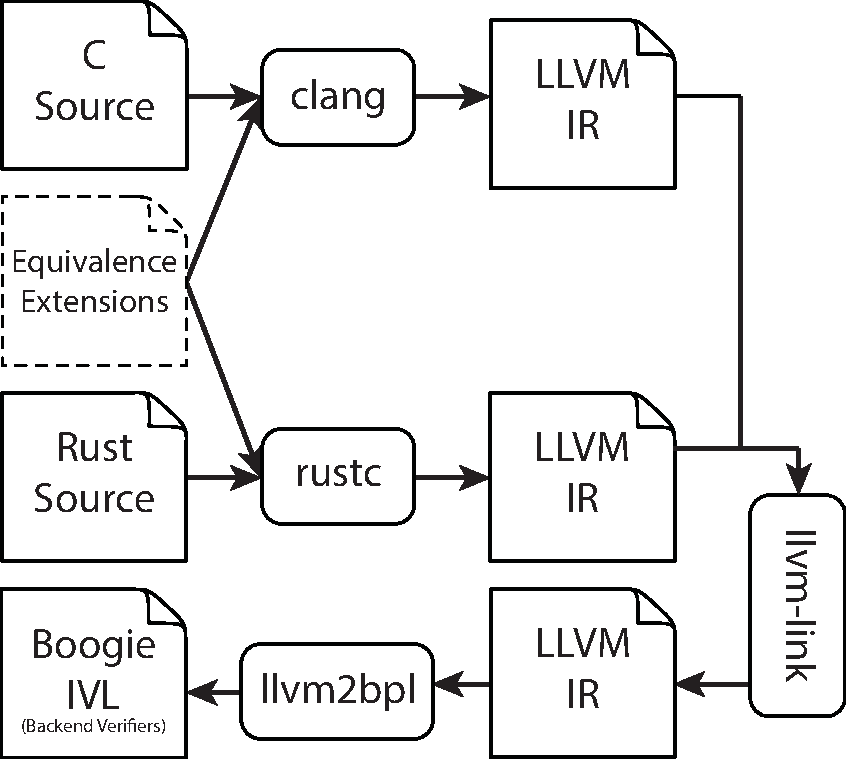
\includegraphics[width=0.92\textwidth]{chap4/fig/SmackEquiv.pdf}
%   \caption{Equivalence checking extensions within SMACK.}
%   \label{fig:toolflow}
% \end{figure}

We added equivalence checking extensions to SMACK, so they are available generally from the tool.
%
These extensions are represented in the ``equivalence extensions'' part of~\cref{fig:toolflow}.
%
The \texttt{verifier\_equiv\_store} functions are implemented in Boogie as shown in~\cref{line:equiv-assume}, where \texttt{\$foeq} is SMACK's floating-point equivalence function corresponding to the SMT-LIB floating-point equality function, \texttt{fp.eq}.
%
We use a global counter \texttt{equiv\_store\\\_counter} to track each value stored in this way.
%
This value is incremented with each use, so as to maintain unique identifiers for retrieving values from \texttt{verifier\_equiv\_store}.
%
This uses the theory of uninterpreted functions to allow the value to effectively be retrieved later.

The \texttt{verifier\_equiv\_check} functions are implemented in Boogie as shown in~\cref{line:equiv-assert} of~\cref{lst:equivstore}.
%
This adds an assertion that the value we are checking is equal to the value stored previously.
%
This also uses a distinct counter to create unique identifiers for the values stored, and increases this value similar to the \texttt{verifier\_equiv\_store} function.
%
The \texttt{verifier\_equiv\_assume} function is implemented similarly.

The use of automatically generated identifiers adds the requirement that uses of \\ \texttt{verifier\_equiv\_check} must occur in the same order and number as uses of \texttt{verifier\\\_equiv\_store}.
%
This is to allow for values inside loops to be checked without associating multiple values to stored values with the same identifier, potentially making the program trivially correct.
%
It is because of this that we introduce the \texttt{verifier\_equiv\_assume} function to allow the user to verify the program, one check at a time.

% \begin{figure}[tb]
% \begin{lstlisting}[label={lst:equivstore}, caption={verifier\_equiv\_store code}, style=boxed, escapechar=`]
% function verifier_store(x: int) returns (float);

% var store_counter: int = 0;
% var load_counter: int = 0;

% procedure verifier_equiv_store(x: float) {`\label{line:equiv-assume}`
%   assume $foeq(x, verifier_store(store_counter));
%   store_counter := store_counter + 1;
% }

% procedure verifier_equiv_check(x: float) {`\label{line:equiv-assert}`
%   assert $foeq(x, verifier_store(load_counter));
%   load_counter := load_counter + 1;
% }
% \end{lstlisting}
% \end{figure}

% \begin{figure}[tb]
% \noindent\begin{minipage}{.47\textwidth}
% \begin{lstlisting}[language=C, label={lst:cstore}, caption={C equivalence}, style=boxed, escapechar=`]
% float c_computation(float x) {
%   float y = 2.0 * x;
%   if(x < -1.0) {
%     y += 1.0;
%     verifier_equiv_store(y);
%   }
%   else if(x <= 0.0) {
%     y -= 1.0;
%     verifier_equiv_store(y);
%   }
%   else if(x <= 1.0) {
%     y *= 2.0;
%     verifier_equiv_store(y);
%   }
%   else {
%     y /= 2.0;
%     verifier_equiv_store(y);
%   }
%   return y;
% }
% \end{lstlisting}
% \end{minipage}
% %
% \begin{minipage}{.52\textwidth}
% \begin{lstlisting}[language=Rust, label={lst:rustequiv}, caption={Rust equivalence}, style=boxed, escapechar=`]
% fn rust_computation(x: f32) -> f32 {
%   let mut y = 2.0 * x;
%   if x < -1.0 {
%     y += 1.0;
%     verifier_equiv_check(y);
%   }
%   else if x <= 0.0 {
%     y -= 1.0;
%     verifier_equiv_check(y);
%   }
%   else if x <= 1.0 {
%     y *= 2.0;
%     verifier_equiv_check(y);
%   }
%   else {
%     y /= 2.0;
%     verifier_equiv_check(y);
%   }
%   return y;
% }
% \end{lstlisting}
% \end{minipage}
% \end{figure}

\subsection{Experiments Using SMT Equivalence}
We investigated the impacts non-equivalence of NaN values has on showing equivalence of expressions in this work.
%
We conducted an experiment where we replaced \\ SMACK's floating-point equivalence functions (\texttt{\$foeq}) as being defined in terms of the SMT equivalence relation, i.e., by defining the \texttt{\$foeq} functions to be the built-in \texttt{=} in Boogie.
%
We used this alternate definition on some of the longer running benchmarks and found they made the assertion checks faster, sometimes by a factor of 10.
%
This suggests that the proof obligation of the solver to show that the expressions are free from NaN values is responsible for some of the scalibility issues we encountered.
%
It should be noted that while there may be some merit in treating NaN values as equivalent only when comparing equality of returned values, this transformation is not sound.
%
For example, the expression \texttt{x != x} should be true when \texttt{x} is NaN.
%
This means that control flow may be affected by treating NaN values as equivalent.
\section{Experiments}

For this work we chose to check the equivalence of the Rust implementation of a
libm by the Rust developers.
%
This library is a native, and idiomatic, Rust language reimplementation of the
\texttt{musl} libm~\cite{musl} library.
%
The \texttt{musl} library provides C-language implementations of IEEE 754 math functions.
%
The version of the \texttt{musl} library used in this work is version 1.1.19.

The Rust libm library is popular, with over fifty million
downloads~\cite{libm-crate} as a package, and it has more than two hundred
dependent packages~\cite{libm-dependents}.
%
This library features the use of for loops, and bit-wise floating-point and
integer operations.
%
The average SLoC is 66.
%
Together, this library has real-world users, has clear targets for verifying
equivalence and are programs of modest size and complexity, and are a good
target on which to use SMACK to check for equivalence.

We have three categories of benchmarks: SMACK-library, basic and advanced.
%
The SMACK-library category includes the functions in the math library that correspond to library functions provided by SMACK.
%
Most of these functions are implemented in terms of SMT solver primitives.
%
For these benchmarks, we also check for equivalence between the Rust, \texttt{musl} and SMACK versions of the functions.
%
This gives an additional benefit of checking that SMACK's math library is correct.

A second category of benchmarks are those that don't require much intervention to verify.
%
The third category is the advanced functions that required advanced methods to help the solver verify, meaning they would take at least an hour to verify.

The functions we worked to verify have several features that influence how hard a program will be for SMACK to verify, and how much manual annotation or modularization 
%
Functions that use bit-wise operations on floating point numbers tend to take longer to verify due to mixing theories, which may limit the solver's ability to use floating-point theory specific reasoning.
%
Functions with multiple branches tend to be slower to prove equivalence due to a lower ability for the solver to detect similar structure between the programs.
%

The basic benchmarks are shown in in~\cref{tab:rustmusl}, the comparison between Rust and SMACK is in~\cref{tab:rustsmack} and the comparison between \texttt{musl} and SMACK is in~\cref{tab:muslsmack}.
%
The advanced benchmarks are shown in~\cref{tab:advancedbench}.

In the basic benchmarks, we can see that Corral with Z3 is the worst performing verifier due to its worse performance on many benchmarks.
%
Boogie with Z3 is the most consistent performing verifier, verifying all but one benchmark in the time limit, which is 1200s.
%

In the comparisons between Rust and SMACK, we see that Boogie with CVC5 is the best performing verifier, solving all queries under the time limit of 1200s.
%
Boogie with Z3 is the next best performing verifier, with Corral behind it.
%
In the comparison between \texttt{musl} and SMACK, all three perform worse.
%
This is notable because the SMACK library versions of these functions are written in C and Boogie.
%
It may be that Rust code is easier for the solver to check equivalence with the Boogie code than it is for C.

In the advanced functions, Boogie with Z3 is the best performing solver, solving all benchmarks in their time limits.
%
Boogie with CVC5 is the next best, solving two benchmarks, then Corral solving no benchmarks.
%
This is partially due to using Boogie with Z3 for gauging the difficulty of equivalence checks, rather than doing the same with Corral or Boogie with CVC5.

All benchmarks were conducted on an Intel 12900ks@5.2GHz, with 16 performance cores and 64GB of memory.
%
The versions of the software used were: Z3 version 4.8.12, CVC5 version 1.0.5, Boogie version 2.9.6 and Corral version 1.1.8.
%
The benchmark suite is available at: \url{https://github.com/keram88/libm-equiv}.
%
The modifications to SMACK are available at: \url{https://github.com/smackers/smack/tree/equiv}
% \begin{table}[!htp]\centering
% \caption{Rust and \texttt{musl} equivalence results}\label{tab:rustmusl}
% \begin{tabular}{lrrrrrrrr}\toprule
% Name &Status & Boogie/CVC5 &Boogie/Z3&Corral&Unroll &Inputs &SLoC \\\midrule
% ceil & Equivalent & TO & 86.4$\pm$1.78s&TO &N/A &(f64) &88 \\
% ceilf &Equivalent & TO &2.2$\pm$0.07s &2.6$\pm$0.03s &N/A &(f32) &76 \\
% copysign &Equivalent & 5.4$\pm$0.51s &1.5$\pm$0.03s &3$\pm$0.06s &N/A &(f64, f64) &15 \\
% copysignf &Equivalent & 2.4$\pm$0.26s &1.4$\pm$0.06s &2.2$\pm$0.06s &N/A &(f32, f32) &17 \\
% fabs &Equivalent & 2.7$\pm$0.22s &1.9$\pm$0.05s &5.6$\pm$0.15s &N/A &(f64) &38 \\
% fabsf &Equivalent & 2.0$\pm$0.19s &1.6$\pm$0.04s &2.5$\pm$0.09s &N/A &(f32) &38 \\
% fdim &Equivalent & 5.8$\pm$0.18s &1.6$\pm$0.04s &9.2$\pm$0.06s &N/A &(f64, f64) &22 \\
% fdimf &Equivalent & 5.0$\pm$0.18s&1.6$\pm$0.03s &3.1$\pm$0.07s &N/A &(f32, f32) &22 \\
% floor &Equivalent & TO & 113.5$\pm$2.85s &TO &N/A &(f64) &87 \\
% floorf &Equivalent &  TO &3.2$\pm$0.07s &3.5$\pm$0.12s &N/A &(f32) &77 \\
% fmax &Equivalent & 4.7$\pm$0.22s &6.2$\pm$0.11s &52.4$\pm$2.69s &N/A &(f64, f64) &15 \\
% fmaxf &Equivalent & 3.3$\pm$0.07s&2.8$\pm$0.11s &7.9$\pm$0.04s &N/A &(f32, f32) &15 \\
% fmin &Equivalent & 4.9$\pm$0.12s &21.5$\pm$0.34s &110.7$\pm$2.96s &N/A &(f64, f64) &15 \\
% fminf &Equivalent & 3.1$\pm$0.18s&7.4$\pm$0.15s &8.8$\pm$0.22s &N/A &(f32, f32) &15 \\
% fmod &Equivalent & TO &22.9$\pm$0.64s &83$\pm$0.91s &2 &(f64, f64) &128 \\
% fmodf &Equivalent & TO &183.4$\pm$3.5s &366.9$\pm$5.12s &2 &(f32, f32) &129 \\
% frexp &Equivalent & TO & 22.8$\pm$0.85s &TO &3 &(f64, i32) &38 \\
% frexpf &Equivalent & TO& 10.5$\pm$0.08s &TO &3 &(f32) &39 \\
% ilogb &Equivalent & 3.0$\pm$0.16s &1.4$\pm$0.09s &2.5$\pm$0.06s &N/A &(f64) &52 \\
% ilogbf &Equivalent & 2.9$\pm$0.17s &1.8$\pm$0.03s &3$\pm$0.1s &N/A &(f32) &52 \\
% modf &Equivalent & TO & 53.2$\pm$0.92s &TO &N/A &(f64) &55 \\
% modff &Equivalent & TO & 60.1$\pm$1.45s &TO &N/A &(f32) &56 \\
% nextafter &Equivalent & TO &44.3$\pm$0.77s &12.3$\pm$0.41s &N/A &(f64, f64) &59 \\
% nextafterf &Equivalent & TO &28.2$\pm$0.21s &11.1$\pm$0.37s &N/A &(f32, f32) &58 \\
% remquo &Equivalent & TO & 210.8$\pm$4.25s &TO &1 &(f64, f64) &164 \\
% remquof &Equivalent & TO & 363.3$\pm$10.35s &TO &2 &(f32, f32) &164 \\
% rint &Equivalent & 7.5$\pm$0.40s &12.1$\pm$0.28s &50.8$\pm$0.69s &N/A &(f64) &68 \\
% rintf &Equivalent & 3.1$\pm$0.15s &5.4$\pm$0.15s &9.9$\pm$0.16s &N/A &(f32) &70 \\
% round & Equivalent & 434$\pm$14.47s&TO &TO &N/A &(f64) &55 \\
% roundf &Equivalent & 61.6$\pm$2.3s &285$\pm$7.25s &237$\pm$6.84s &N/A &(f32) &58 \\
% scalbn &Equivalent & 21.8$\pm$1.45s &207.8$\pm$3.6s &652$\pm$11.79s &N/A &(f64, i32) &58 \\
% scalbnf &Equivalent & 8.2$\pm$0.225s &34.1$\pm$0.64s &62.3$\pm$1.91s &N/A &(f32, i32) &57 \\
% trunc &Equivalent & 6.8$\pm$0.28s & 2.56$\pm$0.05s &TO &N/A &(f64) &50 \\
% truncf &Equivalent & 2.1$\pm$0.11s&25.3$\pm$0.21s &15.1$\pm$0.25s &N/A &(f32) &51 \\
% \bottomrule
% \end{tabular}
% \end{table}\

% \begin{table}[!htp]\centering
% \caption{Rust checked against SMACK}\label{tab:rustsmack}
% \begin{tabular}{lrrrrr}\toprule
% Function Name &Status &Boogie/CVC5 Time &Boogie/Z3 Time &Corral Time \\\midrule
% ceil &Equivalent &1012.3$\pm$22.71s &TO &TO \\
% ceilf &Equivalent &2.2$\pm$0.18s &12.6$\pm$0.89s &4.3$\pm$0.29s \\
% copysign &Equivalent &4.4$\pm$0.11s &2.3$\pm$0.09s &17.4$\pm$0.35s \\
% copysignf &Equivalent &2.2$\pm$0.17s &2$\pm$0.25s &4.4$\pm$0.31s \\
% fabs &Equivalent &2$\pm$0.17s &2.1$\pm$0.08s &2.3$\pm$0.13s \\
% fabsf &Equivalent &1.9$\pm$0.16s &2$\pm$0.26s &2.3$\pm$0.14s \\
% floor &Equivalent &800.3$\pm$78.76s &TO &TO \\
% floorf &Equivalent &2.5$\pm$0.04s &10.9$\pm$0.49s &4.9$\pm$0.26s \\
% fmax &Equivalent &2.1$\pm$0.07s &15.7$\pm$0.16s &TO \\
% fmaxf &Equivalent &2.1$\pm$0.02s &6.8$\pm$0.08s &83.4$\pm$1.01s \\
% fmin &Equivalent &2.1$\pm$0s &61.2$\pm$2.58s &150.9$\pm$1.43s \\
% fminf &Equivalent &2.2$\pm$0.11s &6.6$\pm$0.32s &15.8$\pm$0.31s \\
% fmod &Error (Expected) &590.9$\pm$1.15s &TO &TO \\
% fmodf &Error (Expected) &20.4$\pm$0.38s &113.5$\pm$15.5s &260.5$\pm$4.27s \\
% modf &Equivalent &4.9$\pm$0.05s &132.7$\pm$6.09s &TO \\
% modff &Equivalent &5$\pm$0.03s &52.8$\pm$5.69s &145.2$\pm$9.82s \\
% rint &Equivalent &11.8$\pm$0.06s &302.7$\pm$6.16s &781.8$\pm$186.03s \\
% rintf &Equivalent &3.9$\pm$0.16s &28.3$\pm$1.98s &76$\pm$0.05s \\
% round &Equivalent &5.7$\pm$0.01s &77.8$\pm$2.86s &227.4$\pm$2.14s \\
% roundf &Equivalent &3.2$\pm$0.11s &12.9$\pm$0.47s &62.2$\pm$3.85s \\
% trunc &Equivalent &2.3$\pm$0.12s &62.8$\pm$4.77s &14$\pm$0.04s \\
% truncf &Equivalent &2.2$\pm$0.08s &18.9$\pm$0.73s &3.6$\pm$0.09s \\
% \bottomrule
% \end{tabular}
% \end{table}

% \begin{table}[!htp]\centering
% \caption{musl checked against SMACK}\label{tab:muslsmack}
% \begin{tabular}{lrrrrr}\toprule
% Function Name &Status &Boogie/CVC5 Time &Boogie/Z3 Time &Corral Time \\\midrule
% ceil &TO &TO &TO &TO \\
% ceilf &Equivalent &TO &8$\pm$0.26s &5.6$\pm$0.11s \\
% copysign &Equivalent &9.6$\pm$0.86s &2.7$\pm$0.13s &14.3$\pm$0.41s \\
% copysignf &Equivalent &2.9$\pm$0.21s &2$\pm$0.19s &5.1$\pm$0.14s \\
% fabs &Equivalent &2.5$\pm$0.13s &3.5$\pm$0.12s &6.2$\pm$0.37s \\
% fabsf &Equivalent &2.1$\pm$0.14s &2.1$\pm$0.04s &4.1$\pm$0.25s \\
% floor &TO &TO &TO &TO \\
% floorf &Equivalent &TO &7.5$\pm$0s &5.9$\pm$0.04s \\
% fmax &Equivalent &4.5$\pm$0.2s &2.1$\pm$0.02s &4.2$\pm$0.04s \\
% fmaxf &Equivalent &3.1$\pm$0.1s &2.1$\pm$0.16s &3.6$\pm$0.15s \\
% fmin &Equivalent &4.5$\pm$0.01s &2.1$\pm$0.12s &4$\pm$0.11s \\
% fminf &Equivalent &3.2$\pm$0.13s &2.2$\pm$0.04s &3.7$\pm$0.05s \\
% fmod &Error (Expected) &450.7$\pm$12.14s &TO &TO \\
% fmodf &Error (Expected) &44.2$\pm$2.1s &403.2$\pm$0.59s &TO \\
% modf &TO &TO &TO &TO \\
% modff &TO &TO &TO &TO \\
% rint &Equivalent &21.7$\pm$1.64s &225.9$\pm$29.59s &641.2$\pm$159.96s \\
% rintf &Equivalent &5$\pm$0.13s &32.8$\pm$0.3s &81$\pm$3.81s \\
% round &Equivalent &395.7$\pm$58.92s &TO &TO \\
% roundf &Equivalent &51.3$\pm$0.64s &213.4$\pm$18.85s &795.1$\pm$194.6s \\
% trunc &Equivalent &7.7$\pm$0.32s &12.9$\pm$0.54s &16.1$\pm$0.32s \\
% truncf &Equivalent &3.2$\pm$0.01s &4.4$\pm$0.11s &4.5$\pm$0.15s \\
% \bottomrule
% \end{tabular}
% \end{table}

% \begin{table}[!htp]\centering
% \small
% \caption{Advanced benchmarks}\label{tab:advancedbench}
% \begin{tabular}{lrrrrrrr}\toprule
% Function &Status &Boogie/CVC5 Time &Boogie/Z3 Time &Corral Time &Inputs &SLoC \\\midrule
% acosf &Equivalent &TO &855.6$\pm$17.81s &TO &(f32) &94 \\
% cbrtf &Equivalent &TO &2923.6$\pm$38.05s &TO &(f32) &57 \\
% k\_cos &Equivalent &86.4$\pm$1.61s &14.1$\pm$0.65s &TO &(f64, f64) &27 \\
% k\_cosf &Equivalent &18.4$\pm$0.11s &18.8$\pm$0.8s &TO &(f64) &21 \\
% k\_tanf &Equivalent &TO &30$\pm$0.72s &TO &(f64) &34 \\
% logf &Equivalent &TO &998.3$\pm$15.19s &TO &(f32) &78 \\
% log10f &Equivalent &TO &876.3$\pm$28.17s &TO &(f32) &107 \\
% log2f &Equivalent &TO &1176.9$\pm$29.62s &TO &(f32) &102 \\
% \bottomrule
% \end{tabular}
% \end{table}
\section{Experience}

In this section, we discuss our experience using our modified SMACK tool\-chain.
%
Name\-ly, the discovery of two bugs (one in the Rust math library and one in SMACK's math library) and an example experience using the SMACK extensions for equivalence checking.

\subsection{Bug in the Rust \texttt{nextafter} Function}
While performing equivalence checking between the \texttt{musl} and Rust implementations of the \texttt{nextafter} and \texttt{nextafterf} functions, we discovered an error in Rust's error detection.
%
We will focus on the double precision function \texttt{nextafter} which has the signature \texttt{fn nextafter(x: f64, y: f64) -\textgreater  f64} in Rust.
%
The behavior of this function is to return the next floating-point number after \texttt{x} in the direction of \texttt{y}, e.g., \texttt{nextafter(1.0, 2.0)} returns the smallest floating-point number greater than {\texttt 1.0} and \texttt{nextafter(1.0, 0.0)} returns the largest floating-point number less than \texttt{1.0}.

The IEEE~754 standard for this function~\cite{nextafterieee} specifies error reporting in the case of overflow or underflow.
%
For example, consider the next floating point after \texttt{1.79E+308}\footnote{The full number is \texttt{1.7976931348623157E+308}.} in the direction of \texttt{inf}.
%
Since this is the largest, non-infinite floating point number, the result of \texttt{nextafter(1.79E+308, inf)} is \texttt{inf}.
%
In this situation, the result overflows and the standard says that this should raise the \texttt{FE\_INEXACT} and \texttt{FE\_UNDERFLOW} floating-point exceptions, which may be checked by the user upon return.

We performed variable-wise, equivalence checking between the Rust and \texttt{musl} versions of this program.
%
When we checked the variable \texttt{e} that appears on line 3 of the two programs shown in~\cref{fig:nextaftercrs}, we found that the two programs diverged for some inputs.
%
This calculation is meant to calculate the exponent portion of the result in order to determine if underflow or overflow has occurred.
%
However, the calculation in the Rust version is functionally equivalent to \texttt{ux\_i \textgreater\textgreater (52 \& 0x7ff)}, which is effectively \texttt{ux\_i \textgreater\textgreater 52}.
%
This leaves the sign bit of the exponent intact.
%
The retained sign bit means that if the result is negative, the condition on line 6 of the Rust program will not detect overflow, meaning the computation on line 7 won't generate the requisite inexact and overflow flags.
%
We found a similar error in the calculation of the exponent in the 32-bit version of the function.
%
We reported this issue~\cite{nextafterissue} to the Rust developers and our fixes~\cite{nextafterpr} to this issue was merged into the library.

An interesting aspect with respect to the Rust implementation is that currently
Rust doesn't support accessing the floating-point environment, meaning
floating-point exceptions can't currently be tested in the Rust implementation.
%
This lack of support means that the current tests in the Rust library are not
testing that the correct floating-point exception is raised.
%
However, SMACK can show that there is a control flow divergence that would not
be detected by the library's tests.
%
The current lack of testing means that if Rust supports the floating-point
environment in at some future point, this incorrect code may be used assuming
the code is correct.
%
Because SMACK does not rely on the floating-point environment and can analyze a
programs logical control flow, it can find a bug that testing cannot currently
find.

% \begin{figure}[tbh]
% \begin{minipage}{.50\textwidth}
% \begin{lstlisting}[language=C, label={lst:nextafterc}, caption=nextafter in \texttt{musl}, style=boxed]
% double nextafter(double x, double y) {
%     ...
%     e = ux.i >> 52 & 0x7ff;
%     verifier_store(e,``musl_e'');
%     /* raise overflow if ux.f is
%     infinite and x is finite */
%     if (e == 0x7ff)
%         FORCE_EVAL(x+x);
%     ...
% }
% \end{lstlisting}
% \end{minipage}
% \begin{minipage}{.50\textwidth}
% \begin{lstlisting}[language=Rust, label={lst:nextafterrs}, caption=nextafter in Rust, style=boxed]
% fn nextafter(x:f64, y:f64) {
%     ...
%     let e=ux_i.wrapping_shr(52&0x7ff);
%     verifier_comp(e,``musl_e'');
%     // raise overflow if ux.f is
%     // infinite and x is finite
%     if e == 0x7ff {
%         force_eval!(x + x);
%     }
%     ...
% }
% \end{lstlisting}
% \end{minipage}
% \caption{An example of how SMACK found a control-flow divergence in the implementations for the {\tt nextafter} functions as implemented in C and Rust.}
% \end{figure}

\subsection{Bug in SMACK's Math Library}
In the process of checking the SMACK library functions, we found a bug in SMACK's modeling of the \texttt{copysign} functions in the \texttt{fmod}~\cite{smackfmod} functions.
%
In \cref{lst:smackfmod}, Clang translates the call to \texttt{copysign} to the LLVM intrinsic function \texttt{@llvm.copysign.f32}.
%
SMACK translates this to an undefined uninterpreted-function in Boogie, as it does not model this intrinsic.
%
This means the SMACK library \texttt{fmod} function will return a nondeterministic value, so it is not equivalent to the Rust or \texttt{musl} implementations.
%
This does not apply to comparing the \texttt{copysign} functions in \texttt{musl} and Rust against SMACK since Clang does not modify SMACK's definition.
%
This bug has been submitted to the SMACK developers.

% \begin{lstlisting}[language=C, label={lst:smackfmod}, caption=SMACK's fmod function, style=boxed, escapechar=`]
% double fmod(double x, double y) {
%   ...
%   return copysign(ret, x);`\label{line:fmodcopysign}`
% }
% \end{lstlisting}

\subsection{Verifying Advanced Functions}
Here we describe our experiences verifying two functions from the advanced function category.
\subsubsection{Verifying \texttt{k\_tanf}}
The Rust libm function \texttt{k\_tanf}~(\cref{lst:rustktanf}) corresponds to the \texttt{\_\_kernel\_tandf}~(\cref{lst:muslktanf}) function from \texttt{musl} libm.
%
This function computes the tangent of \texttt{x} to 32-bit precision after range reduction.
%
This function computes intermediate results in 64-bit precision, then returns the final result rounded to 32-bit precision.
%
The function also does not use bit-wise operations.

The function appears straightforward to verify at first; however, it takes more than an hour to check equivalence.
%
Because of the time to verify, this function qualifies for advanced techniques.
%
We applied the guided equivalence checking to verify this function.

To start, we check equivalence of \texttt{r} at~\cref{line:ktanffirstcheck} in~\cref{lst:rustktanf}.
%
As expected, this check times out since it the same as checking the equivalence of the functions themselves.
%
We then add a check at~\cref{line:ktanfseccheck}, while disabling the original check.
%
This equality check can be verified in seconds.
%
We can then add additional checks as shown in~\cref{lst:rustktanf}.
%
While adding new checks, prior, verified checks can be converted to assumes.
%
This allows for the function to be verified incrementally, meaning the current check is the only one being verified.
%
This allows for feedback as to which checks are the most difficult, suggesting they need more work to verify.

Finally, once all checks are completed, any assumed equivalence checks can be returned to being equivalence checks.
%
This allows the entire program to be checked without potentially adding faulty assumptions.
%
In this example, verification can be completed in 27.6s with Boogie as the verifier and Z3 as the solver.
%
This is similar to the total time taken to verify each check individually.

% \begin{lstlisting}[language=Rust, label={lst:rustktanf}, caption=Annotated k\_tanf function from Rust libm, style=boxed, escapechar=`, float=tb]
% fn k_tanf(x: f64, odd: bool) -> f32 {
%     let z = x * x;
%     verifier_equiv_check_f64(z);`\label{line:ktanfseccheck}`
%     let mut r = T[4] + z * T[5];
%     verifier_equiv_check_f64(r);
%     let t = T[2] + z * T[3];
%     verifier_equiv_check_f64(t);
%     let w = z * z;
%     verifier_equiv_check_f64(w);
%     let s = z * x;
%     verifier_equiv_check_f64(s);
%     let u = T[0] + z * T[1];
%     verifier_equiv_check_f64(u);
%     r = (x + s * u) + (s * w) * (t + w * r);
%     verifier_equiv_check_f64(r);`\label{line:ktanffirstcheck}`
%     verifier_equiv_check_f64(-1. / r);
%     (if odd { -1. / r } else { r }) as f32
% }
% fn main() {
%     let x = 1.0f64.verifier_nondet();
%     verifier_assume!(!x.is_nan());
%     let y = 1i32.verifier_nondet();
%     let bsd_res = unsafe { __kernel_tandf(x, y) };
%     let rust_res = k_tanf(x, y != 1);
%     verifier_assert!(bsd_res == rust_res);
% }
% \end{lstlisting}
% \begin{lstlisting}[language=C, label={lst:muslktanf}, caption=Annotated \_\_kernel\_tandf function from \texttt{musl} libm, style=boxed, float=tb]
% __kernel_tandf(double x, int iy)
% {
% 	double z,r,w,s,t,u;

% 	z	=  x*x;
% 	__VERIFIER_equiv_store_double(z);
% 	r = T[4]+z*T[5];
% 	__VERIFIER_equiv_store_double(r);
% 	t = T[2]+z*T[3];
% 	__VERIFIER_equiv_store_double(t);
% 	w = z*z;
% 	__VERIFIER_equiv_store_double(w);
% 	s = z*x;
% 	__VERIFIER_equiv_store_double(s);
% 	u = T[0]+z*T[1];
% 	__VERIFIER_equiv_store_double(u);
% 	r = (x+s*u)+(s*w)*(t+w*r);
% 	__VERIFIER_equiv_store_double(r);
% 	__VERIFIER_equiv_store_double(-1.0/r);
% 	if(iy==1) return r;
% 	else return -1.0/r;
% }
% \end{lstlisting}

\subsubsection{Additional Verification Techniques}
Occasionally, checking equivalence at the variable level can be too slow.
%
The \texttt{acosf} function shown in \cref{lst:rustacosf} demonstrates such a case.
%
Here, the expression at~\cref{line:acosfretexp} times out during verification.
%
We can use a more advanced technique here and break the expression up by checking its sub-expressions.
%
On~\cref{line:acosfsubexp} we see that we can check the second part of the expression.
%
We can continue to do this until we get reasonable verification times for each step.
%
This helps the solver match up more of the sub-expressions, aiding in verification.
%
For this program, this reduced verification time from more than an hour to taking about 15 minutes.

% \begin{lstlisting}[language=Rust, label={lst:rustacosf}, caption=Partially annotated acosf function from Rust libm, style=boxed, escapechar=`, float=tb]
% fn acosf(x: f32) -> f32 {
%     let mut hx = x.to_bits();
%     let ix = hx & 0x7fffffff;
%     ...
%     /* |x| < 0.5 */
%     if ix < 0x3f000000 {
%         if ix <= 0x32800000 {
%             /* |x| < 2**-26 */
%             return PIO2_HI + x1p_120;
%         }
%         verifier_equiv_check_f32(r(x*x));
%         verifier_equiv_check_f32(x*r(x*x));
%         verifier_equiv_check_f32(PIO2_LO - x*r(x*x));
%         verifier_equiv_check_f32(x-(PIO2_LO - x*r(x*x)));`\label{line:acosfsubexp}`
%         verifier_equiv_check_f32(PIO2_HI-(x-(PIO2_LO - x*r(x*x))));
%         return PIO2_HI - (x - (PIO2_LO - x * r(x * x)));`\label{line:acosfretexp}`
%     }
%     ...
% }
% \end{lstlisting}

\subsection{Automatic Porting of C to Rust}
There are tools such as \texttt{c2rust}~\cite{c2rust} which automatically translate C code into Rust code.
%
Such a tool can be used to save the labor of manually translating code, which can be time consuming and can be error prone.
%
While such a translated code is likely to be correct, we can apply SMACK to prove equivalence.

% \begin{lstlisting}[language=C, label={lst:muslcopysign}, caption=Code for the \texttt{copysign} function from \texttt{musl}, style=boxed, escapechar=`, float=tb]
% double copysign(double x, double y) {
% 	union {double f; uint64_t i;} ux={x}, uy={y};
% 	ux.i &= -1ULL/2;
% 	ux.i |= uy.i & 1ULL<<63;
% 	return ux.f;
% }
% \end{lstlisting}

% \begin{lstlisting}[language=Rust, label={lst:c2rustcopysign}, caption=Automatic translation of the \texttt{copysign} function to Rust, style=boxed, escapechar=`, float=tb]
% pub union C2RustUnnamed {
%     pub f: c_double,
%     pub i: c_ulong,
% }
% #[no_mangle]
% pub unsafe extern "C" fn copysign(
%     mut x: c_double,
%     mut y: c_double,
% ) -> c_double {
%     let mut ux = C2RustUnnamed { f: x };
%     let mut uy = C2RustUnnamed { f: y };
%     ux.i = (ux.i as c_ulonglong
%         & (1 as c_ulonglong)
%             .wrapping_neg()
%             .wrapping_div(2 as c_int as c_ulonglong)) as c_ulong;
%     ux.i = (ux.i as c_ulonglong
%         | uy.i as c_ulonglong & (1 as c_ulonglong) << 63 as c_int)
%         as c_ulong;
%     return ux.f;
% }
% \end{lstlisting}

We now explore an example of applying \texttt{c2rust} to a function in the \texttt{musl} library.
%
The code for the \texttt{copysign} function from the \texttt{musl} library is shown in~\cref{lst:muslcopysign}, and its corresponding translation from \texttt{c2rust} is shown in \cref{lst:c2rustcopysign}.
%
We can apply SMACK to show these two programs are equivalent.
%
Once this equivalence has been shown, the C code can be replaced by the Rust code.
%
Because the translated Rust function uses the \textsc{\#[no\_mangle]} attribute, this code can also continue to be used by users of the C langaugae library.

% \begin{lstlisting}[language=Rust, label={lst:rustcopysign}, caption=Idiomatic translation of \texttt{copysign} to Rust, style=boxed, escapechar=`, float=tb]
% pub fn copysign(x: f64, y: f64) -> f64 {
%     let mut ux = x.to_bits();
%     let uy = y.to_bits();
%     ux &= (-1i64 as u64)/2;
%     ux |= uy & (1 << 63);
%     f64::from_bits(ux)
% }
% \end{lstlisting}

One disadvantage of using automatic translation is the code produced may not be idiomatic, nor readable, as seen in \cref{lst:c2rustcopysign}.
%
Because we have already shown the equivalence of the C and translated Rust codes, we can produce an equivalent, idiomatic function in Rust as shown in \cref{lst:rustcopysign}.
%
We can show that this function is equivalent to the one produced by \texttt{c2rust} and by transitivity its equivalence to the original \texttt{musl} code.
%
Because we are now checking equivalence of two programs written in Rust, there are more tools available to prove this equivalence because there is no need for multi-language support.

Here we showed the role that automatic translation can play when porting a library to another programming language.
%
Using this approach, a library can be ported piece-by-piece, and a record of its equivalence to the old language can be maintained.
\section{Related Work}

In SymDiff~\cite{lahiri2012symdiff} the authors looked at making a tool to compute a \textit{symbolic difference} between two versions of the same program.
%
This is done for C programs translated to the Boogie IVL.
%
The SymDiff tool shows portions of code that have identical behavior, while finding semantic differences between the two programs.
%
Because it operates on Boogie IVL, it is possible that SymDiff could be applied to cross-language comparisons.

In~\cite{transval}, a tool K\textsc{eq} based on the $\mathbb{K}$~\cite{ksemfram} which is used to check translation validation of compiled code.
%
In this work, the authors develop a tool to check equivalence of translations from C to LLVM and from LLVM to x86 binary code.
%
This tool uses the $\mathbb{K}$ framework similarly to how SMACK or SymDiff use LLVM IR/Boogie as a common language for verification.
%
Because the use of this common language for verification, the authors are able to do cross-language equivalence checking on code generated by a compiler.
%
This tool could be extended to support cross-language verification as in this work through the use of LLVM IR.

In~\cite{diffkemp} the authors devlop a tool called D\textsc{iff}K\textsc{emp} which is meant to test equivalence of changes made to the Linux kernel and \texttt{musl}.
%
The tool works by trying to apply \textit{semantic-preserving change patterns} to the code to try to show equivalence, rather than using a solver or an intermediate language.
%
This relates to our guided equivalence checking in that in this work it is used to help the solver find the equivalence of the statements.
%
The techniques in this work could benefit this tool by automatically identifying portions of the C and Rust programs which may be equivalent.
%
This would allow for more scalable verification and less user intervention.

In~\cite{ucklee} a tool based on the \textsc{klee} system, named \textsc{uc-klee}, is developed to check equivalence of functions.
%
The \textsc{klee} system is a symbolic execution which is based on LLVM IR.
%
\textsc{uc-klee} adds equivalence checking extensions which automate making input variables non-deterministic and checking returned values are equal.
%
This work is limited to checking equivalence of functions in one language, but it could be extended to support cross-language verification.

\section{Conclusions}
In this work we showed that SMACK could be used as a practical tool to do equivalence checking between C and Rust programs.
%
We showed that SMACK can find bugs in these programs that may not otherwise be detectable.
%
The floating-point and bit-vector theories proved to be a scalability challenge.
%
We developed techniques to address some of these challenges with varying degrees of success.
%
The equivalence checking extensions made to SMACK made the best improvements to SMACK's scalability, albeit with additional labor.
%
These extensions can be used in the future to do equivalence checking on new libraries, possibly ported between languages.


\bibliographystyle{plain}
\bibliography{refs}
\newpage
\begin{figure}[H]
\noindent\begin{minipage}[t]{.49\textwidth}
% \begin{lstlisting}[language=Rust, label={lst:rustfivex}, caption={Rust code}, style=boxed, escapechar=`, basicstyle=\small]
\begin{lstlisting}[language=Rust, style=boxed, escapechar=`, basicstyle=\small]
fn rust_five_x(x: f32) -> f32 {`\label{line:rustfivex}`
  return 5.0*x;
}
extern "C" {
  fn c_five_x(x: f32) -> f32;
}
fn main() {`\label{line:fivexharness}`
  let x = 0.0.verifier_nondet();`\label{line:xcreate}`
  verifier_assume!(!isnan(x));`\label{line:xconstrain}`
  let c_res = unsafe {c_five_x(x)};`\label{line:fivexccall}`
  let rust_res = rust_five_x(x);`\label{line:fivexrustcall}`
  verifier_assert!(c_res==rust_res);`\label{line:fivexassert}`
}
\end{lstlisting}
\end{minipage}
%
\begin{minipage}[t]{.49\textwidth}
%\begin{lstlisting}[language=C, label={lst:cfivex}, caption={C code}, style=boxed, escapechar=`, basicstyle=\small]
\begin{lstlisting}[language=C, style=boxed, escapechar=`, basicstyle=\small]
float c_five_x(float x) {`\label{line:cfivex}`
  return x+x+x+x+x;
}
\end{lstlisting}
\end{minipage}
\caption{An example of a Rust program (left) that checks the equivalence of a native Rust-language function and an external C-language function (right).}
\label{fig:rustcfivex}
\end{figure}

%%%%%%%%%%%%%%%%%%%%%%%%%%%%%%%%%%%%%%%%%%%%%%%%%%%%%%%%%%%%%%%%%%%%%%%%%%%%%%%%%%%%%%%%%

\begin{figure}[H]
\noindent\begin{minipage}{.49\textwidth}
%\begin{lstlisting}[frame=tb, language=Rust, label={lst:rustsixx}, caption={Rust code.}, style=boxed, escapechar=`, basicstyle=\small]
\begin{lstlisting}[frame=tb, language=Rust, style=boxed, escapechar=`, basicstyle=\small]
fn rust_six_x(x: f32) -> f32 {`\label{line:rustsixx}`
  return 6.0*x;
}
\end{lstlisting}
\end{minipage}
%
\begin{minipage}{.49\textwidth}
%\begin{lstlisting}[frame=tb, language=C, label={lst:csixx}, caption={C Code.}, style=boxed, escapechar=`, basicstyle=\small]
\begin{lstlisting}[frame=tb, language=C, style=boxed, escapechar=`, basicstyle=\small]
float c_six_x(float x) {`\label{line:csixx}`
  return x+x+x+x+x+x;
}
\end{lstlisting}
\end{minipage}
\caption{An example of a program written in Rust (left) and a program written in C (right) which may seem to be equivalent.}
\label{fig:crustsixx}
\end{figure}

%%%%%%%%%%%%%%%%%%%%%%%%%%%%%%%%%%%%%%%%%%%%%%%%%%%%%%%%%%%%%%%%%%%%%%%%%%%%%%%%%%%%%%%%%

\begin{figure}[H]
\noindent\begin{minipage}{.47\textwidth}
%\begin{lstlisting}[language=C, label={lst:cstore}, caption={C equivalence.}, style=boxed, escapechar=`]
\begin{lstlisting}[language=C, style=boxed, escapechar=`]
float c_computation(float x) {
  float y = 2.0 * x;
  if(x < -1.0) {
    y += 1.0;
    verifier_equiv_store(y);
  }
  else if(x <= 0.0) {
    y -= 1.0;
    verifier_equiv_store(y);
  }
  else if(x <= 1.0) {
    y *= 2.0;
    verifier_equiv_store(y);
  }
  else {
    y /= 2.0;
    verifier_equiv_store(y);
  }
  return y;
}
\end{lstlisting}
\end{minipage}
%
\begin{minipage}{.52\textwidth}
\begin{lstlisting}[language=Rust, style=boxed, escapechar=`]
fn rust_computation(x: f32) -> f32 {
  let mut y = 2.0 * x;
  if x < -1.0 {
    y += 1.0;
    verifier_equiv_check(y);
  }
  else if x <= 0.0 {
    y -= 1.0;
    verifier_equiv_check(y);
  }
  else if x <= 1.0 {
    y *= 2.0;
    verifier_equiv_check(y);
  }
  else {
    y /= 2.0;
    verifier_equiv_check(y);
  }
  return y;
}
\end{lstlisting}
\end{minipage}
\caption{A demonstration of how the equivalence checking extensions to SMACK are used to verify equivalence of these C-language and Rust-language programs (left and right, respectively).}
\label{fig:storeequiv}
\end{figure}

%%%%%%%%%%%%%%%%%%%%%%%%%%%%%%%%%%%%%%%%%%%%%%%%%%%%%%%%%%%%%%%%%%%%%%%%%%%%%%%%%%%%%%%%%

\begin{figure}[H]
  \centering
  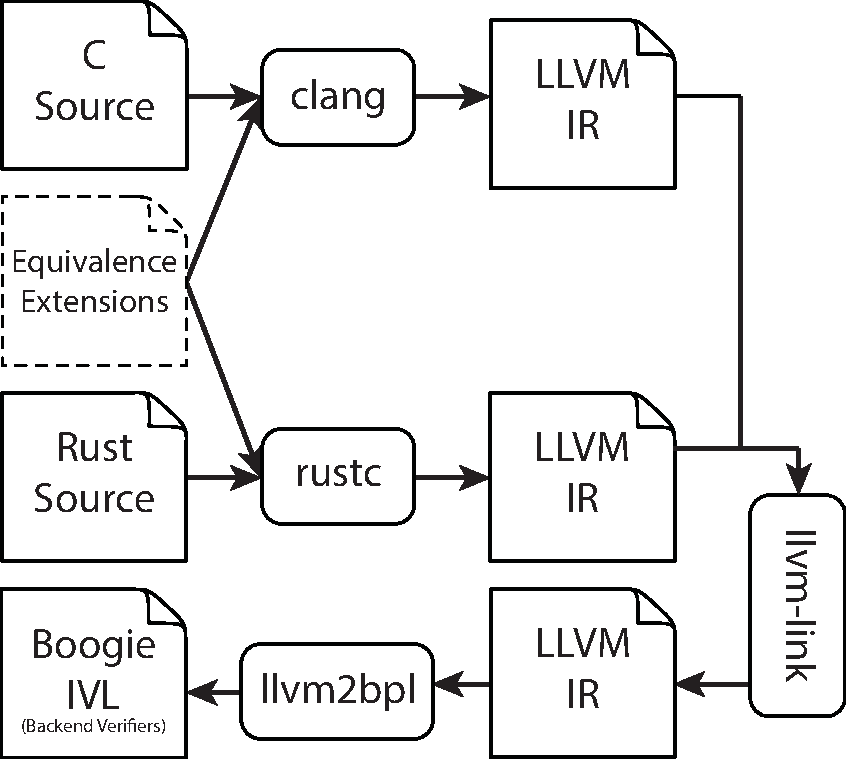
\includegraphics[width=0.92\textwidth]{chap4/fig/SmackEquiv.pdf}
  \caption{Equivalence checking extensions within SMACK.}
  \label{fig:toolflow}
\end{figure}

%%%%%%%%%%%%%%%%%%%%%%%%%%%%%%%%%%%%%%%%%%%%%%%%%%%%%%%%%%%%%%%%%%%%%%%%%%%%%%%%%%%%%%%%%

\begin{figure}[H]
\begin{minipage}[t]{.50\textwidth}
%\begin{lstlisting}[language=C, label={lst:nextafterc}, caption=nextafter in \texttt{musl}, style=boxed]
\begin{lstlisting}[language=C, style=boxed]
double nextafter(double x,
                 double y) {
    ...
    e = ux.i >> 52 & 0x7ff;
    verifier_store(e,``musl_e'');
    /* raise overflow if ux.f is
    infinite and x is finite */
    if (e == 0x7ff)
        FORCE_EVAL(x+x);
    ...
}
\end{lstlisting}
\end{minipage}
\begin{minipage}[t]{.50\textwidth}
%\begin{lstlisting}[language=Rust, label={lst:nextafterrs}, caption=nextafter in Rust, style=boxed]
\begin{lstlisting}[language=Rust, style=boxed]
fn nextafter(x:f64, y:f64) {
    ...
    let e=ux_i.
         wrapping_shr(52&0x7ff);
    verifier_comp(e,``musl_e'');
    // raise overflow if ux.f is
    // infinite and x is finite
    if e == 0x7ff {
        force_eval!(x + x);
    }
    ...
}
\end{lstlisting}
\end{minipage}
\caption{An example of how SMACK found a control-flow divergence in the implementations for the {\tt nextafter} functions as implemented in C (left) and Rust (right).}
\label{fig:nextaftercrs}
\end{figure}

%%%%%%%%%%%%%%%%%%%%%%%%%%%%%%%%%%%%%%%%%%%%%%%%%%%%%%%%%%%%%%%%%%%%%%%%%%%%%%%%%%%%%%%%%

\begin{table}[H]\centering
\caption{Rust and \texttt{musl} equivalence results.}\label{tab:rustmusl}
\vspace{1em}
\resizebox{\columnwidth}{!}{
\begin{tabular}{lrrrrrrrr}\toprule
Name &Status & Boogie/CVC5 &Boogie/Z3&Corral&Unroll &Inputs &SLoC \\\midrule
ceil & Equivalent & TO & 86.4$\pm$1.78s&TO &N/A &(f64) &88 \\
ceilf &Equivalent & TO &2.2$\pm$0.07s &2.6$\pm$0.03s &N/A &(f32) &76 \\
copysign &Equivalent & 5.4$\pm$0.51s &1.5$\pm$0.03s &3$\pm$0.06s &N/A &(f64, f64) &15 \\
copysignf &Equivalent & 2.4$\pm$0.26s &1.4$\pm$0.06s &2.2$\pm$0.06s &N/A &(f32, f32) &17 \\
fabs &Equivalent & 2.7$\pm$0.22s &1.9$\pm$0.05s &5.6$\pm$0.15s &N/A &(f64) &38 \\
fabsf &Equivalent & 2.0$\pm$0.19s &1.6$\pm$0.04s &2.5$\pm$0.09s &N/A &(f32) &38 \\
fdim &Equivalent & 5.8$\pm$0.18s &1.6$\pm$0.04s &9.2$\pm$0.06s &N/A &(f64, f64) &22 \\
fdimf &Equivalent & 5.0$\pm$0.18s&1.6$\pm$0.03s &3.1$\pm$0.07s &N/A &(f32, f32) &22 \\
floor &Equivalent & TO & 113.5$\pm$2.85s &TO &N/A &(f64) &87 \\
floorf &Equivalent &  TO &3.2$\pm$0.07s &3.5$\pm$0.12s &N/A &(f32) &77 \\
fmax &Equivalent & 4.7$\pm$0.22s &6.2$\pm$0.11s &52.4$\pm$2.69s &N/A &(f64, f64) &15 \\
fmaxf &Equivalent & 3.3$\pm$0.07s&2.8$\pm$0.11s &7.9$\pm$0.04s &N/A &(f32, f32) &15 \\
fmin &Equivalent & 4.9$\pm$0.12s &21.5$\pm$0.34s &110.7$\pm$2.96s &N/A &(f64, f64) &15 \\
fminf &Equivalent & 3.1$\pm$0.18s&7.4$\pm$0.15s &8.8$\pm$0.22s &N/A &(f32, f32) &15 \\
fmod &Equivalent & TO &22.9$\pm$0.64s &83$\pm$0.91s &2 &(f64, f64) &128 \\
fmodf &Equivalent & TO &183.4$\pm$3.5s &366.9$\pm$5.12s &2 &(f32, f32) &129 \\
frexp &Equivalent & TO & 22.8$\pm$0.85s &TO &3 &(f64, i32) &38 \\
frexpf &Equivalent & TO& 10.5$\pm$0.08s &TO &3 &(f32) &39 \\
ilogb &Equivalent & 3.0$\pm$0.16s &1.4$\pm$0.09s &2.5$\pm$0.06s &N/A &(f64) &52 \\
ilogbf &Equivalent & 2.9$\pm$0.17s &1.8$\pm$0.03s &3$\pm$0.1s &N/A &(f32) &52 \\
modf &Equivalent & TO & 53.2$\pm$0.92s &TO &N/A &(f64) &55 \\
modff &Equivalent & TO & 60.1$\pm$1.45s &TO &N/A &(f32) &56 \\
nextafter &Equivalent & TO &44.3$\pm$0.77s &12.3$\pm$0.41s &N/A &(f64, f64) &59 \\
nextafterf &Equivalent & TO &28.2$\pm$0.21s &11.1$\pm$0.37s &N/A &(f32, f32) &58 \\
remquo &Equivalent & TO & 210.8$\pm$4.25s &TO &1 &(f64, f64) &164 \\
remquof &Equivalent & TO & 363.3$\pm$10.35s &TO &2 &(f32, f32) &164 \\
rint &Equivalent & 7.5$\pm$0.40s &12.1$\pm$0.28s &50.8$\pm$0.69s &N/A &(f64) &68 \\
rintf &Equivalent & 3.1$\pm$0.15s &5.4$\pm$0.15s &9.9$\pm$0.16s &N/A &(f32) &70 \\
round & Equivalent & 434$\pm$14.47s&TO &TO &N/A &(f64) &55 \\
roundf &Equivalent & 61.6$\pm$2.3s &285$\pm$7.25s &237$\pm$6.84s &N/A &(f32) &58 \\
scalbn &Equivalent & 21.8$\pm$1.45s &207.8$\pm$3.6s &652$\pm$11.79s &N/A &(f64, i32) &58 \\
scalbnf &Equivalent & 8.2$\pm$0.225s &34.1$\pm$0.64s &62.3$\pm$1.91s &N/A &(f32, i32) &57 \\
trunc &Equivalent & 6.8$\pm$0.28s & 2.56$\pm$0.05s &TO &N/A &(f64) &50 \\
truncf &Equivalent & 2.1$\pm$0.11s&25.3$\pm$0.21s &15.1$\pm$0.25s &N/A &(f32) &51 \\
\bottomrule
\end{tabular}
}
\end{table}

%%%%%%%%%%%%%%%%%%%%%%%%%%%%%%%%%%%%%%%%%%%%%%%%%%%%%%%%%%%%%%%%%%%%%%%%%%%%%%%%%%%%%%%%%

\begin{table}[H]\centering
\caption{Rust checked against SMACK.}\label{tab:rustsmack}
\vspace{1em}
\resizebox{\columnwidth}{!}{
\begin{tabular}{lrrrrr}\toprule
Function Name &Status &Boogie/CVC5 Time &Boogie/Z3 Time &Corral Time \\\midrule
ceil &Equivalent &1012.3$\pm$22.71s &TO &TO \\
ceilf &Equivalent &2.2$\pm$0.18s &12.6$\pm$0.89s &4.3$\pm$0.29s \\
copysign &Equivalent &4.4$\pm$0.11s &2.3$\pm$0.09s &17.4$\pm$0.35s \\
copysignf &Equivalent &2.2$\pm$0.17s &2$\pm$0.25s &4.4$\pm$0.31s \\
fabs &Equivalent &2$\pm$0.17s &2.1$\pm$0.08s &2.3$\pm$0.13s \\
fabsf &Equivalent &1.9$\pm$0.16s &2$\pm$0.26s &2.3$\pm$0.14s \\
floor &Equivalent &800.3$\pm$78.76s &TO &TO \\
floorf &Equivalent &2.5$\pm$0.04s &10.9$\pm$0.49s &4.9$\pm$0.26s \\
fmax &Equivalent &2.1$\pm$0.07s &15.7$\pm$0.16s &TO \\
fmaxf &Equivalent &2.1$\pm$0.02s &6.8$\pm$0.08s &83.4$\pm$1.01s \\
fmin &Equivalent &2.1$\pm$0s &61.2$\pm$2.58s &150.9$\pm$1.43s \\
fminf &Equivalent &2.2$\pm$0.11s &6.6$\pm$0.32s &15.8$\pm$0.31s \\
fmod &Error (Expected) &590.9$\pm$1.15s &TO &TO \\
fmodf &Error (Expected) &20.4$\pm$0.38s &113.5$\pm$15.5s &260.5$\pm$4.27s \\
modf &Equivalent &4.9$\pm$0.05s &132.7$\pm$6.09s &TO \\
modff &Equivalent &5$\pm$0.03s &52.8$\pm$5.69s &145.2$\pm$9.82s \\
rint &Equivalent &11.8$\pm$0.06s &302.7$\pm$6.16s &781.8$\pm$186.03s \\
rintf &Equivalent &3.9$\pm$0.16s &28.3$\pm$1.98s &76$\pm$0.05s \\
round &Equivalent &5.7$\pm$0.01s &77.8$\pm$2.86s &227.4$\pm$2.14s \\
roundf &Equivalent &3.2$\pm$0.11s &12.9$\pm$0.47s &62.2$\pm$3.85s \\
trunc &Equivalent &2.3$\pm$0.12s &62.8$\pm$4.77s &14$\pm$0.04s \\
truncf &Equivalent &2.2$\pm$0.08s &18.9$\pm$0.73s &3.6$\pm$0.09s \\
\bottomrule
\end{tabular}
}
\end{table}

%%%%%%%%%%%%%%%%%%%%%%%%%%%%%%%%%%%%%%%%%%%%%%%%%%%%%%%%%%%%%%%%%%%%%%%%%%%%%%%%%%%%%%%%%

\begin{table}[H]\centering
\caption{\texttt{musl} checked against SMACK.}\label{tab:muslsmack}
\vspace{1em}
\resizebox{\columnwidth}{!}{
\begin{tabular}{lrrrrr}\toprule
Function Name &Status &Boogie/CVC5 Time &Boogie/Z3 Time &Corral Time \\\midrule
ceil &TO &TO &TO &TO \\
ceilf &Equivalent &TO &8$\pm$0.26s &5.6$\pm$0.11s \\
copysign &Equivalent &9.6$\pm$0.86s &2.7$\pm$0.13s &14.3$\pm$0.41s \\
copysignf &Equivalent &2.9$\pm$0.21s &2$\pm$0.19s &5.1$\pm$0.14s \\
fabs &Equivalent &2.5$\pm$0.13s &3.5$\pm$0.12s &6.2$\pm$0.37s \\
fabsf &Equivalent &2.1$\pm$0.14s &2.1$\pm$0.04s &4.1$\pm$0.25s \\
floor &TO &TO &TO &TO \\
floorf &Equivalent &TO &7.5$\pm$0s &5.9$\pm$0.04s \\
fmax &Equivalent &4.5$\pm$0.2s &2.1$\pm$0.02s &4.2$\pm$0.04s \\
fmaxf &Equivalent &3.1$\pm$0.1s &2.1$\pm$0.16s &3.6$\pm$0.15s \\
fmin &Equivalent &4.5$\pm$0.01s &2.1$\pm$0.12s &4$\pm$0.11s \\
fminf &Equivalent &3.2$\pm$0.13s &2.2$\pm$0.04s &3.7$\pm$0.05s \\
fmod &Error (Expected) &450.7$\pm$12.14s &TO &TO \\
fmodf &Error (Expected) &44.2$\pm$2.1s &403.2$\pm$0.59s &TO \\
modf &TO &TO &TO &TO \\
modff &TO &TO &TO &TO \\
rint &Equivalent &21.7$\pm$1.64s &225.9$\pm$29.59s &641.2$\pm$159.96s \\
rintf &Equivalent &5$\pm$0.13s &32.8$\pm$0.3s &81$\pm$3.81s \\
round &Equivalent &395.7$\pm$58.92s &TO &TO \\
roundf &Equivalent &51.3$\pm$0.64s &213.4$\pm$18.85s &795.1$\pm$194.6s \\
trunc &Equivalent &7.7$\pm$0.32s &12.9$\pm$0.54s &16.1$\pm$0.32s \\
truncf &Equivalent &3.2$\pm$0.01s &4.4$\pm$0.11s &4.5$\pm$0.15s \\
\bottomrule
\end{tabular}
}
\end{table}

%%%%%%%%%%%%%%%%%%%%%%%%%%%%%%%%%%%%%%%%%%%%%%%%%%%%%%%%%%%%%%%%%%%%%%%%%%%%%%%%%%%%%%%%%

\begin{table}[H]\centering
\small
\caption{Advanced benchmarks.}\label{tab:advancedbench}
\vspace{1em}
\resizebox{\columnwidth}{!}{
\begin{tabular}{lrrrrrrr}\toprule
Function &Status &Boogie/CVC5 Time &Boogie/Z3 Time &Corral Time &Inputs &SLoC \\\midrule
acosf &Equivalent &TO &855.6$\pm$17.81s &TO &(f32) &94 \\
cbrtf &Equivalent &TO &2923.6$\pm$38.05s &TO &(f32) &57 \\
k\_cos &Equivalent &86.4$\pm$1.61s &14.1$\pm$0.65s &TO &(f64, f64) &27 \\
k\_cosf &Equivalent &18.4$\pm$0.11s &18.8$\pm$0.8s &TO &(f64) &21 \\
k\_tanf &Equivalent &TO &30$\pm$0.72s &TO &(f64) &34 \\
logf &Equivalent &TO &998.3$\pm$15.19s &TO &(f32) &78 \\
log10f &Equivalent &TO &876.3$\pm$28.17s &TO &(f32) &107 \\
log2f &Equivalent &TO &1176.9$\pm$29.62s &TO &(f32) &102 \\
\bottomrule
\end{tabular}
}
\end{table}

%%%%%%%%%%%%%%%%%%%%%%%%%%%%%%%%%%%%%%%%%%%%%%%%%%%%%%%%%%%%%%%%%%%%%%%%%%%%%%%%%%%%%%%%%

% \begin{lstlisting}[style=boxed, escapechar=`]
\begin{lstlisting}[label={lst:equivstore}, caption={Boogie code implementing verifier\_equiv\_store.}, style=boxed, escapechar=`, captionpos=b, float=tbh]
function verifier_store(x: int) returns (float);

var store_counter: int = 0;
var load_counter: int = 0;

procedure verifier_equiv_store(x: float) {`\label{line:equiv-assume}`
  assume $foeq(x, verifier_store(store_counter));
  store_counter := store_counter + 1;
}

procedure verifier_equiv_check(x: float) {`\label{line:equiv-assert}`
  assert $foeq(x, verifier_store(load_counter));
  load_counter := load_counter + 1;
}
\end{lstlisting}
% \caption{Boogie code implementing verifier\_equiv\_store.}
% \label{lst:equivstore}
% \end{figure}

%%%%%%%%%%%%%%%%%%%%%%%%%%%%%%%%%%%%%%%%%%%%%%%%%%%%%%%%%%%%%%%%%%%%%%%%%%%%%%%%%%%%%%%%%

% \begin{figure}
% \begin{lstlisting}[language=C,style=boxed, escapechar=`]
\begin{lstlisting}[language=C, label={lst:smackfmod}, caption={Implementation of SMACK's fmod function.}, style=boxed, escapechar=`, captionpos=b, float=tbh]
double fmod(double x, double y) {
  ...
  return copysign(ret, x);`\label{line:fmodcopysign}`
}
\end{lstlisting}
% \caption{Implementation of SMACK's fmod function.}
% \label{lst:smackfmod}
% \end{figure}

%%%%%%%%%%%%%%%%%%%%%%%%%%%%%%%%%%%%%%%%%%%%%%%%%%%%%%%%%%%%%%%%%%%%%%%%%%%%%%%%%%%%%%%%%
% \begin{figure}
% \begin{lstlisting}[language=Rust, style=boxed, escapechar=`]
\begin{lstlisting}[language=Rust, label={lst:rustktanf}, caption=Annotated k\_tanf function from Rust libm., style=boxed, escapechar=`, float=tbh, captionpos=b]
fn k_tanf(x: f64, odd: bool) -> f32 {
    let z = x * x;
    verifier_equiv_check_f64(z);`\label{line:ktanfseccheck}`
    let mut r = T[4] + z * T[5];
    verifier_equiv_check_f64(r);
    let t = T[2] + z * T[3];
    verifier_equiv_check_f64(t);
    let w = z * z;
    verifier_equiv_check_f64(w);
    let s = z * x;
    verifier_equiv_check_f64(s);
    let u = T[0] + z * T[1];
    verifier_equiv_check_f64(u);
    r = (x + s * u) + (s * w) * (t + w * r);
    verifier_equiv_check_f64(r);`\label{line:ktanffirstcheck}`
    verifier_equiv_check_f64(-1. / r);
    (if odd { -1. / r } else { r }) as f32
}
fn main() {
    let x = 1.0f64.verifier_nondet();
    verifier_assume!(!x.is_nan());
    let y = 1i32.verifier_nondet();
    let bsd_res = unsafe { __kernel_tandf(x, y) };
    let rust_res = k_tanf(x, y != 1);
    verifier_assert!(bsd_res == rust_res);
}
\end{lstlisting}
% \caption{Annotated k\_tanf function from Rust libm.}
% \label{lst:rustktanf}
% \end{figure}

%%%%%%%%%%%%%%%%%%%%%%%%%%%%%%%%%%%%%%%%%%%%%%%%%%%%%%%%%%%%%%%%%%%%%%%%%%%%%%%%%%%%%%%%%
\begin{figure}[tbh]
\vspace{10em}
\begin{lstlisting}[language=C, label={lst:muslktanf}, caption=Annotated \_\_kernel\_tandf function from \texttt{musl} libm., style=boxed, captionpos=b]
__kernel_tandf(double x, int iy)
{
	double z,r,w,s,t,u;

	z	=  x*x;
	__VERIFIER_equiv_store_double(z);
	r = T[4]+z*T[5];
	__VERIFIER_equiv_store_double(r);
	t = T[2]+z*T[3];
	__VERIFIER_equiv_store_double(t);
	w = z*z;
	__VERIFIER_equiv_store_double(w);
	s = z*x;
	__VERIFIER_equiv_store_double(s);
	u = T[0]+z*T[1];
	__VERIFIER_equiv_store_double(u);
	r = (x+s*u)+(s*w)*(t+w*r);
	__VERIFIER_equiv_store_double(r);
	__VERIFIER_equiv_store_double(-1.0/r);
	if(iy==1) return r;
	else return -1.0/r;
}
\end{lstlisting}
\vspace{10em}
\end{figure}
%%%%%%%%%%%%%%%%%%%%%%%%%%%%%%%%%%%%%%%%%%%%%%%%%%%%%%%%%%%%%%%%%%%%%%%%%%%%%%%%%%%%%%%%%

\begin{lstlisting}[language=Rust, label={lst:rustacosf}, caption=Partially annotated acosf function from Rust libm., style=boxed, escapechar=`, float=tbh, captionpos=b]
fn acosf(x: f32) -> f32 {
    let mut hx = x.to_bits();
    let ix = hx & 0x7fffffff;
    ...
    /* |x| < 0.5 */
    if ix < 0x3f000000 {
        if ix <= 0x32800000 {
            /* |x| < 2**-26 */
            return PIO2_HI + x1p_120;
        }
        verifier_equiv_check_f32(r(x*x));
        verifier_equiv_check_f32(x*r(x*x));
        verifier_equiv_check_f32(PIO2_LO - x*r(x*x));
        verifier_equiv_check_f32(x-(PIO2_LO - x*r(x*x)));`\label{line:acosfsubexp}`
        verifier_equiv_check_f32(PIO2_HI-(x-(PIO2_LO - x*r(x*x))));
        return PIO2_HI - (x - (PIO2_LO - x * r(x * x)));`\label{line:acosfretexp}`
    }
    ...
}
\end{lstlisting}

%%%%%%%%%%%%%%%%%%%%%%%%%%%%%%%%%%%%%%%%%%%%%%%%%%%%%%%%%%%%%%%%%%%%%%%%%%%%%%%%%%%%%%%%%

\begin{lstlisting}[language=C, label={lst:muslcopysign}, caption=Code for the \texttt{copysign} function from \texttt{musl}., style=boxed, escapechar=`, float=tbh, captionpos=b]
double copysign(double x, double y) {
	union {double f; uint64_t i;} ux={x}, uy={y};
	ux.i &= -1ULL/2;
	ux.i |= uy.i & 1ULL<<63;
	return ux.f;
}
\end{lstlisting}

%%%%%%%%%%%%%%%%%%%%%%%%%%%%%%%%%%%%%%%%%%%%%%%%%%%%%%%%%%%%%%%%%%%%%%%%%%%%%%%%%%%%%%%%%

\begin{lstlisting}[language=Rust, label={lst:c2rustcopysign}, caption=Automatic translation of the \texttt{copysign} function to Rust., style=boxed, escapechar=`, float=tbh, captionpos=b]
pub union C2RustUnnamed {
    pub f: c_double,
    pub i: c_ulong,
}
#[no_mangle]
pub unsafe extern "C" fn copysign(
    mut x: c_double,
    mut y: c_double,
) -> c_double {
    let mut ux = C2RustUnnamed { f: x };
    let mut uy = C2RustUnnamed { f: y };
    ux.i = (ux.i as c_ulonglong
        & (1 as c_ulonglong)
            .wrapping_neg()
            .wrapping_div(2 as c_int as c_ulonglong)) as c_ulong;
    ux.i = (ux.i as c_ulonglong
        | uy.i as c_ulonglong & (1 as c_ulonglong) << 63 as c_int)
        as c_ulong;
    return ux.f;
}
\end{lstlisting}

%%%%%%%%%%%%%%%%%%%%%%%%%%%%%%%%%%%%%%%%%%%%%%%%%%%%%%%%%%%%%%%%%%%%%%%%%%%%%%%%%%%%%%%%%

\begin{lstlisting}[language=Rust, label={lst:rustcopysign}, caption=Idiomatic translation of \texttt{copysign} to Rust., style=boxed, escapechar=`, float=tbh, captionpos=b]
pub fn copysign(x: f64, y: f64) -> f64 {
    let mut ux = x.to_bits();
    let uy = y.to_bits();
    ux &= (-1i64 as u64)/2;
    ux |= uy & (1 << 63);
    f64::from_bits(ux)
}
\end{lstlisting}

%%%%%%%%%%%%%%%%%%%%%%%%%%%%%%%%%%%%%%%%%%%%%%%%%%%%%%%%%%%%%%%%%%%%%%%%%%%%%%%%%%%%%%%%%


% \end{document}
